\section{Diskussion}
\label{sec:Diskussion}

\subsection{Diskussion der Ergebnisse}
\label{subsec:diskErg}
Beim Aufbau ist anzumerken, dass die Fließgeschwindigkeit durch den kleinen Radius des Schlauches eventuell beinträchtigt werden könnte.
Dieser könnte zu stark gebogen oder sogar geknickt sein, sodass die Flüssigkeit nicht ausreichend fließen kann.
Außerdem konnte der Schlauch nicht an das Acryl mit den drei einzustellenden Winkeln gedrückt werden, da die Kunststoffplatte nicht 
unter den Schlauch passte und somit nicht für eine bessere Fixierung untergeschoben werden konnte.\newline
Im ersten Teil des Versuches konnten genaue Messwerte erfasst werden und eine grafische Auswertung dieser ergibt die zu erwartende lineare Abhängigkeit
zwischen dem Quotienten $\sfrac{\upDelta\nu}{\cos(\alpha)}$ und der Fließgeschwindigkeit $v$.
Aus der grafischen Auswertung folgt, dass es keinen Zusammenhang zwischen dem Dopplerwinkel und der Strömungsgeschwindigkeit gibt.\newline
Der zweite Teil des Versuches ergab jedoch keine gebrauchbaren Messwerte. Dies liegt vermutlich an der Einstellung des Ultraschall-Doppler Generators.
Es war allerdings nicht möglich den Fehler, der die Werte so stark verzerrte, zu finden. Zu erwarten war, dass die Fließgeschwindigkeit mit der Tiefe zunimmt
und ein Maximum erreicht, wenn der Ultraschall auf der Tiefe der zu untersuchenden Flüssigkeit angekommen ist. Danach hätte die gemessen 
Fließgeschwindigkeit wieder abnehmen sollen. Für die Signalintensität hätte sich eine quadratische Verteilung ergeben sollen.\newline
In unserem Versuch ergaben sich keine deutlichen Werte und es gab kein deutlich abzulesendes Maximum. Wie in \autoref{fig:plot2} und in \autoref{fig:plot3} zu sehen ist, sind
die Werte für die Signalintensität nicht quadratisch verteilt, weshalb naheliegt, dass bei der Einstellung am Messprogramm \textit{Flow View} ein Fehler unterlaufen ist.
In \autoref{fig:plot2} stieg die momentane Fließgeschwindigkeit auch nicht an, was eine Auswertung der Messwerte unmöglich macht. In \autoref{fig:plot3} folgt sie dann auch keinem 
konkreten Verlauf, auch keinen konstanten, mehr. Auch verschiedene Einstellungen des Ultraschall-Generators und des aufzeichnenden Programmes ergaben keine besseren Messwerte.
Es ist deshalb zu sagen, dass der zweite Teil des Versuches nicht auszuwerten ist.\newline

\subsection{Diskussion der Fehlerquellen}
\label{subsec:diskFehler}
Eine mögliche Fehlerquelle ist das Programm \textit{Flow View}, in dem die angezeigten Werte für die Maximal- und Minimalfrequenz $f_{\text{max}},\, \,f_{\text{mean}}$
starken Schwankungen unterlagen. Es war demnach nicht möglich einen genauen Wert abzulesen, wodurch die dadurch bestimmte Frequenzdifferenz ebenfalls
hohen Schwankungen unterliegt.
Eine weitere Fehlerquelle könnte die Menge des verwendeten Ultraschallgels sein. Da hier jedoch mehrere Male mit unterschiedlichen Mengen versucht wurde, Messwerte
zu erstellen und die Qualität nicht besser wurde, ist davon auszugehen, dass zumindest dieser Fehler gering gehalten wurde.
Die Strömungsgeschwindigkeit, die von der Pumpe erzeugt wurde, unterlag ebenfalls hohen Schwankungen. Es war nicht möglich eine genaue Pumpleistung
einzustellen, da bereits durch Erschütterungen des Tisches, auf dem die Pumpe stand, zu einer anderen Pumpleistung führte.
All diese Ungenauigkeiten führten zu schlechteren Messwerten. Jedoch bleibt immer noch offen, weshalb die Messwerte im zweiten Versuchsteil so unbrauchbar sind.

\printbibliography{}


\section*{Anhang}
\label{sec:Anhang}
\begin{figure}
    \centering
    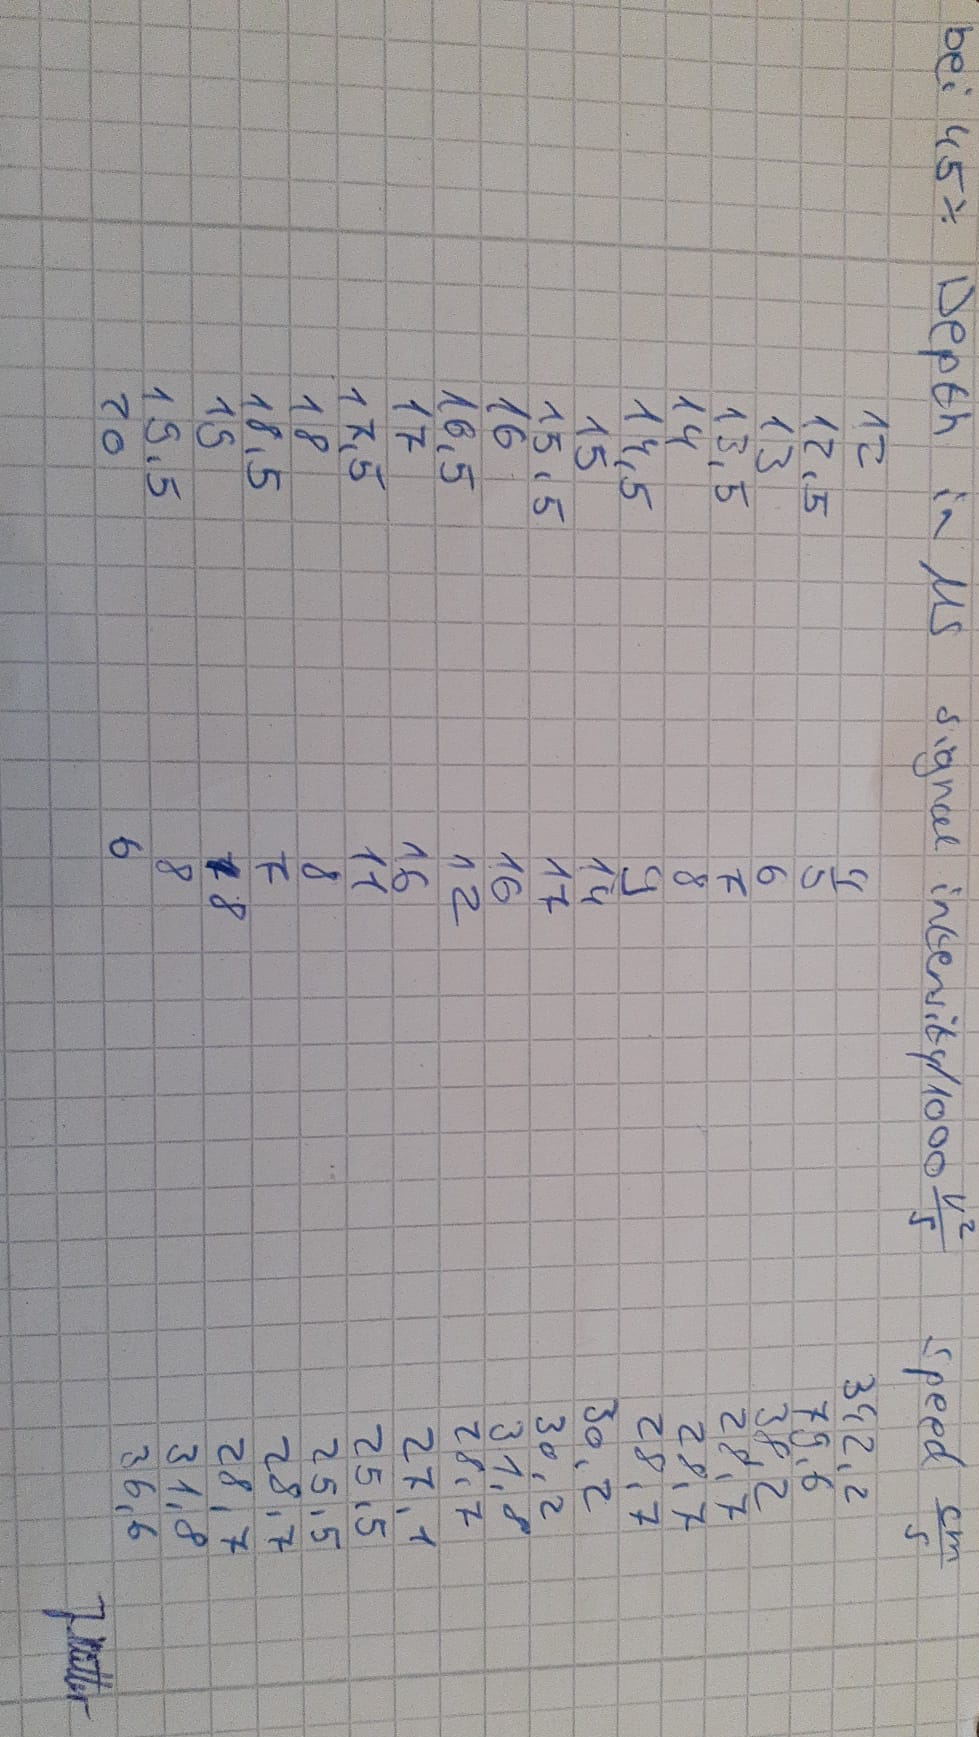
\includegraphics[angle=90, width=0.75\textwidth]{data/origDaten2.png}
    \caption{Originale Messwerte des Versuches.}
    \label{fig:origDaten2}
\end{figure}
\begin{figure}
    \centering
    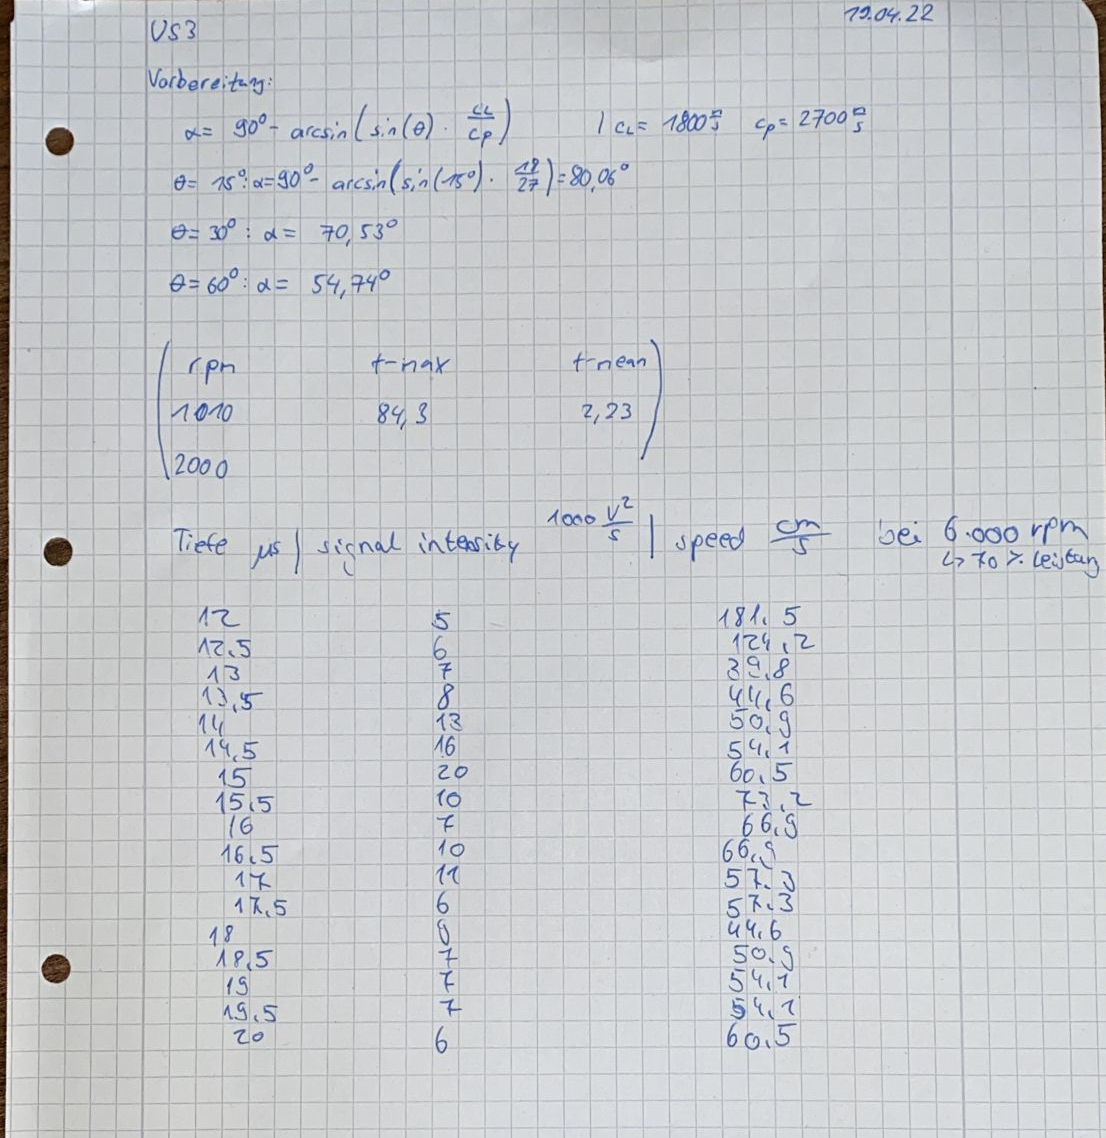
\includegraphics[width=0.75\textwidth]{data/origDaten1.png}
    \caption{Originale Messwerte des Versuches.}
    \label{fig:origDaten1}
\end{figure}
